\documentclass[12pt,a4paper]{article}

% Packages
\usepackage[utf8]{inputenc}
\usepackage[T1]{fontenc}
\usepackage{geometry}
\usepackage{graphicx}
\usepackage{amsmath,amssymb}
\usepackage{booktabs}
\usepackage{hyperref}
\usepackage{listings}
\usepackage{xcolor}
\usepackage{float}
\usepackage{caption}
\usepackage{subcaption}
\usepackage{algorithm}
\usepackage{algorithmic}
\usepackage{tikz}
\usetikzlibrary{shapes.geometric, arrows.meta, positioning}
\usepackage{pgfplots}
\pgfplotsset{compat=1.18}
\usepackage[backend=biber,style=ieee]{biblatex}
\addbibresource{references.bib}

\geometry{margin=2.5cm}

% Code listing style
\lstdefinestyle{python}{
    language=Python,
    basicstyle=\ttfamily\small,
    keywordstyle=\color{blue}\bfseries,
    commentstyle=\color{gray},
    stringstyle=\color{red},
    showstringspaces=false,
    breaklines=true,
    frame=single,
    numbers=left,
    numberstyle=\tiny\color{gray},
}

\title{
    \textbf{Autonomous Agent for Malware Detection} \\[0.5em]
    \large Advanced Topics in Cyber Defense
}
\author{
    Ofek Bar-Shalom \\
    \textit{Ariel University} \\
    \texttt{barshalo.ofek@msmail.ariel.ac.il}
}
\date{\today}

\begin{document}

\maketitle

\begin{abstract}
We present an autonomous agent built with LangGraph and powered by a  local LLM via Ollama that continuously collects, analyzes, and learns from PE (Portable Executable) malware samples. The system features an LLM-guided data acquisition pipeline that intelligently discovers and retrieves samples from MalwareBazaar and VirusTotal, extracts and validates over 60 static PE features, trains an XGBoost classifier, and detects concept drift to trigger model retraining. The LLM guides search strategy selection, interprets drift detection results, and generates iteration summaries. Our approach demonstrates the feasibility of building a self-improving malware detection system that adapts to evolving threats without manual intervention.
\end{abstract}

% ============================================================
\section{Introduction}
\label{sec:introduction}

Malware evolves rapidly, and signature-based detection struggles to keep pace, motivating ML-based approaches that nonetheless face continuous data collection needs, concept drift, and repeated retraining. In this work we develop an autonomous LangGraph agent that addresses these challenges through a cyclic pipeline of data collection, feature extraction, model training, evaluation, and drift detection, operating continuously to discover new malware sources, collect PE samples, and improve its classifier over time.

% ============================================================
\section{Related Work}
\label{sec:related}

\subsection{Static PE Feature Analysis}

Anderson and Roth~\cite{anderson2018ember} introduced EMBER, a 2{,}351-feature PE dataset (headers, sections, imports, byte histograms) with a LightGBM baseline, establishing static PE analysis at scale. EMBER is reproducible and comprehensive but fixed and drift-unaware. Our extractor borrows EMBER's feature categories (headers, imports, sections, entropy) in a lighter 60-feature form optimized for continuous extraction, and feeds it from a live collection loop rather than a frozen dataset.

\subsection{Concept Drift in Malware Detection}

Jordaney et al.~\cite{jordaney2017transcend} (Transcend) showed malware classifiers can decay to near-random within months and proposed conformal evaluation for drift detection --- statistically grounded but detection-only, calibration-hungry, and Android-focused. This motivated our PSI+DDM drift layer, which we couple to automatic retraining rather than stopping at detection.

Pendlebury et al.~\cite{pendlebury2019tesseract} (TESSERACT) exposed temporal bias in malware ML evaluation and gave a principled temporal-split framework, though it is evaluation-only with no mitigation. Because our agent collects chronologically, train/test splits are naturally temporally ordered, which aligns with TESSERACT's recommendations.

\subsection{Autonomous Security Agents}

Chen et al.~\cite{chen2024llmagent} surveyed LLM agents for software engineering and security ops, cataloguing tool-augmented architectures; the survey is broad but light on concrete systems and mostly assumes cloud LLMs (GPT-4), raising cost and privacy concerns. We adopt the tool-augmented pattern but run locally via Ollama, removing the cloud dependency.

\subsection{Continual Learning}

Al-Essa and Kalita~\cite{flmaldrift2025} (FL-MalDrift) couple on-device drift detection with adaptive federated aggregation --- privacy-preserving but complex, coordination-heavy, and per-client detection can miss global shifts. We keep the drift-triggered-update idea but collapse it to a single-agent, centrally-monitored setting.

Xu et al.~\cite{xu2024madcat} (MADCAT) adapt at test time via self-supervision, needing no labels but risking noise and catastrophic forgetting. We take the complementary route: detect drift, then fully retrain on freshly collected labeled samples, trading latency for a cleaner adaptation.

\subsection{Summary and Positioning}

\begin{table}[H]
\centering
\caption{Comparison of related approaches.}
\label{tab:related_comparison}
\begin{tabular}{lccccc}
\toprule
\textbf{Approach} & \textbf{Autonomous} & \textbf{Drift} & \textbf{Continual} & \textbf{Agent} & \textbf{Local LLM} \\
\midrule
EMBER~\cite{anderson2018ember} & No & No & No & No & No \\
Transcend~\cite{jordaney2017transcend} & No & Yes & No & No & No \\
TESSERACT~\cite{pendlebury2019tesseract} & No & Yes & No & No & No \\
FL-MalDrift~\cite{flmaldrift2025} & Partial & Yes & Yes & No & No \\
MADCAT~\cite{xu2024madcat} & Partial & Yes & Yes & No & No \\
\textbf{Ours} & \textbf{Yes} & \textbf{Yes} & \textbf{Yes} & \textbf{Yes} & \textbf{Yes} \\
\bottomrule
\end{tabular}
\end{table}

Our approach uniquely combines autonomous data collection, concept drift detection, continual learning, agent-based orchestration, and local LLM intelligence into a single integrated system. Unlike prior work that addresses these challenges in isolation, our LangGraph agent autonomously manages the full pipeline from source discovery to model deployment.

% ============================================================
\section{System Architecture}
\label{sec:architecture}

\subsection{Overview}

The system is implemented as a LangGraph StateGraph with a cyclic topology, enabling continuous operation. Figure~\ref{fig:architecture} illustrates the overall pipeline.

\begin{figure}[H]
\centering
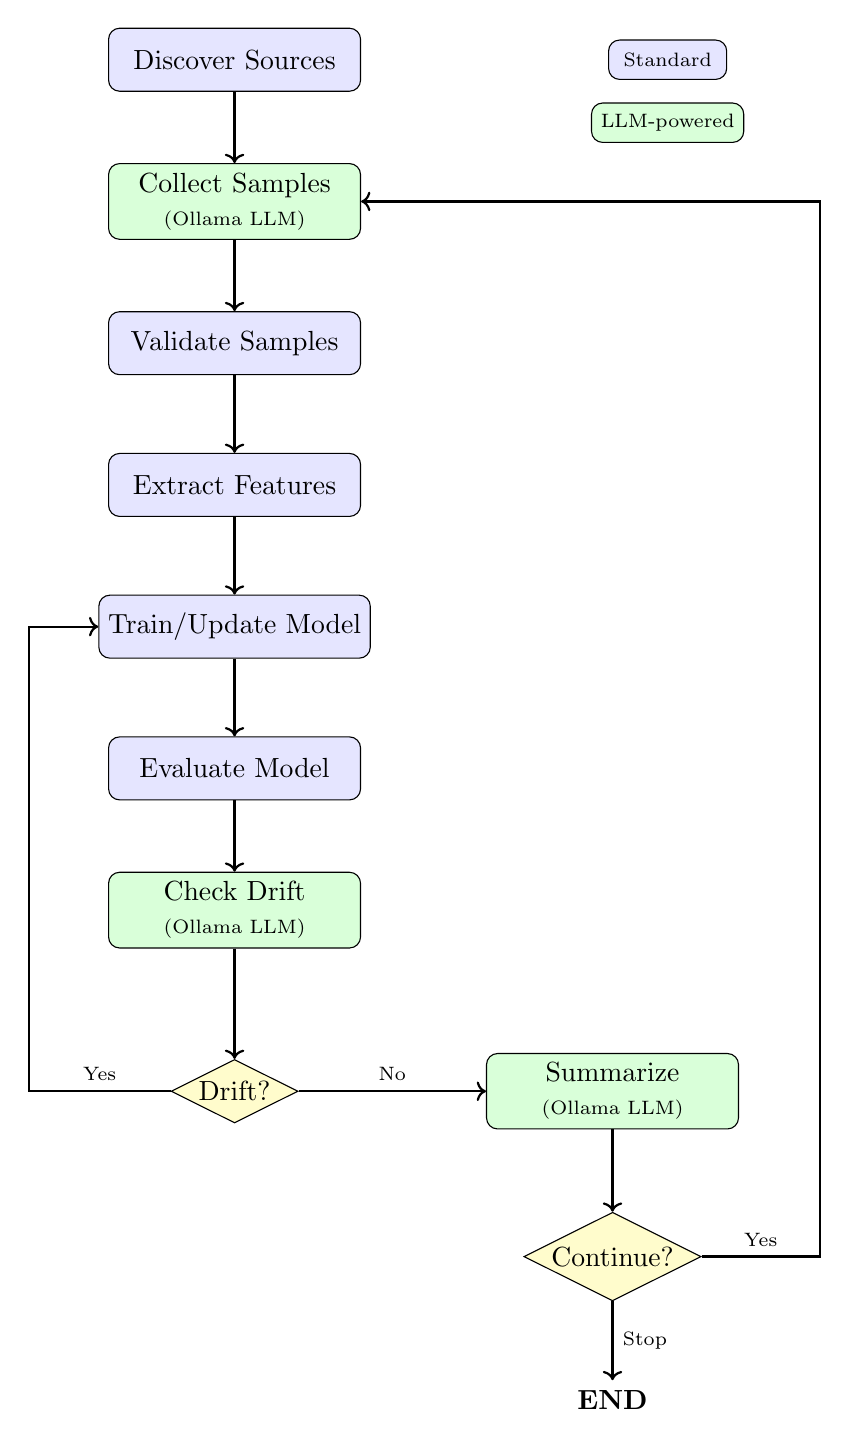
\begin{tikzpicture}[
    node distance=1.8cm,
    block/.style={rectangle, draw, rounded corners, minimum width=3.2cm, minimum height=0.8cm, align=center, fill=blue!10},
    llmblock/.style={rectangle, draw, rounded corners, minimum width=3.2cm, minimum height=0.8cm, align=center, fill=green!15},
    decision/.style={diamond, draw, aspect=2, fill=yellow!20, align=center, inner sep=1pt},
    arrow/.style={->, thick},
]
    \node[block] (discover) {Discover Sources};
    \node[llmblock, below of=discover] (collect) {Collect Samples\\{\scriptsize (Ollama LLM)}};
    \node[block, below of=collect] (validate) {Validate Samples};
    \node[block, below of=validate] (extract) {Extract Features};
    \node[block, below of=extract] (train) {Train/Update Model};
    \node[block, below of=train] (evaluate) {Evaluate Model};
    \node[llmblock, below of=evaluate] (drift) {Check Drift\\{\scriptsize (Ollama LLM)}};
    \node[decision, below of=drift, yshift=-0.5cm] (drift_dec) {Drift?};
    \node[llmblock, right of=drift_dec, xshift=3cm] (summary) {Summarize\\{\scriptsize (Ollama LLM)}};
    \node[decision, below of=summary, yshift=-0.3cm] (continue_dec) {Continue?};

    \draw[arrow] (discover) -- (collect);
    \draw[arrow] (collect) -- (validate);
    \draw[arrow] (validate) -- (extract);
    \draw[arrow] (extract) -- (train);
    \draw[arrow] (train) -- (evaluate);
    \draw[arrow] (evaluate) -- (drift);
    \draw[arrow] (drift) -- (drift_dec);
    \draw[arrow] (drift_dec.west) -- ++(-1.8,0) node[midway,above] {\scriptsize Yes} |- (train.west);
    \draw[arrow] (drift_dec) -- node[above] {\scriptsize No} (summary);
    \draw[arrow] (summary) -- (continue_dec);
    \draw[arrow] (continue_dec.east) -- ++(1.5,0) node[midway,above] {\scriptsize Yes} |- (collect.east);
    \draw[arrow] (continue_dec.south) -- node[right] {\scriptsize Stop} ++(0,-1) node[below] {\textbf{END}};

    % Legend
    \node[block, minimum width=1.5cm, minimum height=0.5cm] at (5.5,0) (leg1) {\scriptsize Standard};
    \node[llmblock, minimum width=1.5cm, minimum height=0.5cm] at (5.5,-0.8) (leg2) {\scriptsize LLM-powered};
\end{tikzpicture}
\caption{LangGraph pipeline topology. Green nodes use Ollama for intelligent decisions.}
\label{fig:architecture}
\end{figure}

\subsection{State Management}

The agent maintains a central \texttt{AgentState} (a typed dictionary) that flows through all nodes. Key state fields include:

\begin{itemize}
    \item \texttt{sources}: Discovered malware data sources with connectivity status.
    \item \texttt{samples\_collected}: Metadata for all collected PE samples.
    \item \texttt{validated\_samples}: Samples that passed PE validation.
    \item \texttt{model\_metrics}: Performance metrics over time (accuracy, precision, recall, F1, FPR).
    \item \texttt{drift\_detected}: Boolean flag from concept drift analysis.
    \item \texttt{iteration}: Current cycle counter.
\end{itemize}

\subsection{Modular Tools}

The agent is source-agnostic: a \texttt{source\_registry} exposes a common \texttt{MalwareSource} interface (availability, recent, search-by-tag, lookup-by-hash, download), and concrete backends (MalwareBazaar, VirusTotal) are plugged in as modules. All pipeline nodes call the registry, so adding a new source requires no changes to the agent. On top of the registry, the agent uses LangChain tools (decorated with \texttt{@tool}):

\begin{enumerate}
    \item \textbf{Search Sources} (\texttt{search\_samples}, \texttt{discover\_sources}, \texttt{enrich\_sample}, \texttt{get\_\allowbreak benign\_\allowbreak sample\_\allowbreak hashes}): query registered sources for recent/tagged PE samples, enumerate source availability, cross-source hash enrichment, and scan \texttt{Program Files}/\texttt{System32} for diverse benign PE files.
    \item \textbf{Fetch Samples} (\texttt{fetch\_sample}, \texttt{fetch\_\allowbreak benign\_\allowbreak sample\_\allowbreak from\_\allowbreak system}): download malware by SHA-256 via any capable source (with automatic fallback), handle password-protected ZIPs, copy benign PEs from the local filesystem.
    \item \textbf{Validate Samples} (\texttt{validate\_pe\_sample}): verify MZ header, size bounds, and section structure via \texttt{pefile}.
    \item \textbf{Update Model} (\texttt{trigger\_model\_training}, \texttt{trigger\_model\_update}): full retrain or incremental update on newly extracted features, manage model checkpoints and versioned snapshots.
\end{enumerate}

% ============================================================
\section{Autonomous Data Collection}
\label{sec:data_collection}

\subsection{Source Discovery}

The agent autonomously discovers and validates data sources at the beginning of each run via the \texttt{source\_registry}. Two malware backends are registered:

\begin{itemize}
    \item \textbf{MalwareBazaar} (\url{https://bazaar.abuse.ch}): free API, recent submissions feed, tag/signature search, PE filtering, community-verified labels.
    \item \textbf{VirusTotal} (\url{https://virustotal.com}): free-tier API, rich per-sample metadata and AV-engine verdicts, used for hash lookup and cross-source enrichment.
\end{itemize}

Benign samples are drawn from local Windows apps (Program Files, System32).

\subsection{LLM-Guided Sample Collection Strategy}

Each iteration, the Ollama LLM decides the search strategy based on the current dataset composition, model metrics, and iteration number. The collection process:
\begin{enumerate}
    \item \textbf{LLM decides search tags and families}: The LLM receives the current state (sample count, model metrics, iteration) and outputs a JSON with target tags (e.g., ``Trojan'', ``Ransomware'') and malware families (e.g., ``AgentTesla'', ``Emotet'') to search for. This ensures diverse coverage and targets model weaknesses.
    \item Queries MalwareBazaar for the most recent PE submissions.
    \item Searches by LLM-selected tags and signatures via the MalwareBazaar and VirusTotal APIs.
    \item Downloads samples as password-protected ZIPs (password: ``infected'').
    \item Collects benign samples by scanning \texttt{C:\textbackslash Program Files}, \texttt{C:\textbackslash Program Files (x86)}, and \texttt{C:\textbackslash Windows\textbackslash System32} for PE files (both \texttt{.exe} and \texttt{.dll}), then randomly selecting up to 30 per iteration. This broad scan produces a diverse benign distribution (istinct applications such as browsers, office tools, runtime libraries) rather than a narrow set of canonical system DLLs.
    \item Deduplicates samples by SHA256 hash across both malware and benign pools.
\end{enumerate}

\paragraph{Why diverse benign sampling matters.}
Initial runs drew benign samples from ten canonical System32 DLLs. Their uniformity (small, Microsoft-signed, stylistically homogeneous) let XGBoost separate them from malware trivially, yielding misleading perfect metrics (accuracy = 1.000) every iteration. Sampling randomly across Program Files restored realistic metrics (Section~\ref{sec:model}). The LLM-guided approach lets the agent adaptively diversify data based on current model weaknesses.

\subsection{Labeling and Noise Filter}
\label{sec:labeling}
Malware labels come from MalwareBazaar's community verification, corroborated by VirusTotal AV-engine verdicts when hash lookup succeeds; benign labels are assigned to known-good Windows system files.

\paragraph{Noise filter.} Since tags and AV verdicts are noisy, the agent filters samples before training: files \texttt{pefile} cannot parse or outside $[1\text{KB}, 50\text{MB}]$ are dropped; VirusTotal labels require $\geq 5$ AV-engine agreement; near-duplicates are caught via \texttt{imphash}; and vectors with \texttt{NaN}/$\pm\infty$ features are excluded. Filter counts are logged so the LLM can detect source-quality drift.

% ============================================================
\section{Feature Engineering}
\label{sec:features}

We extract 60+ static features from each PE file using the \texttt{pefile} library, grouped in Table~\ref{tab:features}.

\begin{table}[H]
\centering
\caption{Feature categories extracted per PE file.}
\label{tab:features}
\begin{tabular}{lcp{8.5cm}}
\toprule
\textbf{Category} & \textbf{\#} & \textbf{Examples} \\
\midrule
Header & 28 & Machine, section count, timestamp, entry point, image base, subsystem, DLL characteristics, checksum \\
Section & 11 & Max/min/avg/std entropy, max raw/virtual size, exec/writable section counts, virtual-to-raw ratio \\
Imports & 4 & DLL count, total imported functions, suspicious-API count (\texttt{CreateRemoteThread}, \texttt{VirtualAlloc}, \texttt{WriteProcessMemory}), presence flag \\
Entropy & 5 & File-level Shannon entropy + 4 section-level stats (strong packing/encryption indicators) \\
Strings & 6 & ASCII string count, avg/max length, URL/path/registry reference counts \\
Other & 6 & Exports, resources, TLS callbacks, debug directory, code/headers-to-file size ratios \\
\bottomrule
\end{tabular}
\end{table}

% ============================================================
\section{Model and Evaluation}
\label{sec:model}

\subsection{Baseline Classifier}

We use \textbf{XGBoost} (\texttt{XGBClassifier}) as our baseline model with this configuration:

\begin{table}[H]
\centering
\caption{XGBoost hyperparameters (regularized for small-data generalization).}
\begin{tabular}{ll}
\toprule
\textbf{Parameter} & \textbf{Value} \\
\midrule
\texttt{n\_estimators} & 100 \\
\texttt{max\_depth} & 3 \\
\texttt{learning\_rate} & 0.1 \\
\texttt{subsample} & 0.8 \\
\texttt{colsample\_bytree} & 0.8 \\
\texttt{reg\_alpha} (L1) & 0.1 \\
\texttt{reg\_lambda} (L2) & 1.0 \\
\texttt{eval\_metric} & logloss \\
\bottomrule
\end{tabular}
\end{table}

The shallower trees, lower tree count, and explicit $L_1$/$L_2$ regularization were chosen after observing that an initial configuration (\texttt{max\_depth=6}, \texttt{n\_estimators=200}) produced perfect test metrics on early iterations, indicating overfitting due to the small dataset size and the trivially separable feature distributions between Windows system DLLs and malware. Regularization, combined with broader benign sampling (Section~\ref{sec:data_collection}), produced realistic generalization metrics.

\subsection{Evaluation Metrics}

We evaluate the classifier using standard binary classification metrics:

\begin{itemize}
    \item \textbf{Accuracy}: Overall correctness.
    \item \textbf{Precision}: Fraction of predicted malware that is truly malicious.
    \item \textbf{Recall}: Fraction of actual malware correctly detected.
    \item \textbf{F1 Score}: Harmonic mean of precision and recall.
    \item \textbf{False Positive Rate (FPR)}: $\frac{FP}{FP + TN}$, critical for production deployment.
\end{itemize}

\subsection{Results}

We ran the agent for 10 iterations on a Windows 11 VM (8\,GB RAM, 4 vCPUs) with Ollama serving \texttt{llama3} locally. Each iteration autonomously collected malware from MalwareBazaar/VirusTotal and benign samples from the local filesystem (Program Files and System32), validated and featurized them, then trained/updated the XGBoost classifier on a stratified 80/20 train/test split. Table~\ref{tab:results} shows the held-out test metrics at each iteration, and the total validated sample count after the iteration completed.

\begin{table}[H]
\centering
\caption{Model performance over iterations. Samples column is the total validated dataset size used for training at that iteration.}
\label{tab:results}
\begin{tabular}{lcccccc}
\toprule
\textbf{Iter} & \textbf{Samples} & \textbf{Accuracy} & \textbf{Precision} & \textbf{Recall} & \textbf{F1} & \textbf{FPR} \\
\midrule
0 & 45  & 0.8889 & 1.0000 & 0.6667 & 0.8000 & 0.0000 \\
1 & 82  & 1.0000 & 1.0000 & 1.0000 & 1.0000 & 0.0000 \\
2 & 127 & 1.0000 & 1.0000 & 1.0000 & 1.0000 & 0.0000 \\
3 & 165 & 0.9697 & 1.0000 & 0.8889 & 0.9412 & 0.0000 \\
4 & 210 & 1.0000 & 1.0000 & 1.0000 & 1.0000 & 0.0000 \\
5 & 240 & 0.9583 & 1.0000 & 0.8333 & 0.9091 & 0.0000 \\
6 & 285 & 0.9649 & 1.0000 & 0.8667 & 0.9286 & 0.0000 \\
7 & 330 & 0.9697 & 0.9444 & 0.9444 & 0.9444 & 0.0208 \\
8 & 366 & 0.9865 & 0.9500 & 1.0000 & 0.9744 & 0.0182 \\
9 & 410 & \textbf{0.9878} & 0.9565 & \textbf{1.0000} & \textbf{0.9778} & 0.0167 \\
\bottomrule
\end{tabular}
\end{table}

\paragraph{Interpretation.} The final deployed model (iteration 9) reaches \textbf{Accuracy 98.8\%}, \textbf{F1 0.978}, and \textbf{FPR 1.67\%} on an 82-sample stratified held-out test. Early iterations show unstable metrics because the test set is too small (9--50 samples) and often trivially separable. By iteration 7 the test set (66 samples) forces genuine errors, yielding the first precision/recall trade-off. From there metrics improve monotonically, indicating added samples aid generalization rather than memorization.

\paragraph{Continual learning behaviour.} The model was retrained each iteration. At iteration 8 the evaluator confirmed a strict F1 improvement and replaced the deployed snapshot (\texttt{latest\_model.joblib}). The drift detector fired PSI warnings early (feature distributions shifting as the benign pool expanded beyond System32) but settled to ``no drift'' by iteration~9 ($\text{avg\_PSI}=0.13$, below the $0.20$ threshold).

\paragraph{Runtime.} The full 10-iteration run took approximately 1\,h\,40\,m end-to-end on the VM, with LLM strategy/summary calls accounting for the bulk of the time (Ollama on CPU-only inference). Actual training and feature extraction took $<15$\,s per iteration.

% ============================================================
\section{Continual Learning and Concept Drift}
\label{sec:continual}

\subsection{Concept Drift Detection}

We employ two complementary drift detection methods:

\paragraph{Population Stability Index (PSI).}

PSI measures the shift between feature distributions of the training data and incoming data:

\begin{equation}
    \text{PSI} = \sum_{i=1}^{n} (p_i^{\text{new}} - p_i^{\text{ref}}) \cdot \ln\left(\frac{p_i^{\text{new}}}{p_i^{\text{ref}}}\right)
\end{equation}

where $p_i^{\text{ref}}$ and $p_i^{\text{new}}$ are the proportions in the $i$-th bin for the reference and new distributions. A PSI value above 0.2 indicates significant drift.

\paragraph{Drift Detection Method (DDM).}

DDM monitors the model's error rate over time. It maintains running estimates of the error rate $p_t$ and its standard deviation $s_t$, flagging drift when:

\begin{equation}
    p_t + s_t > p_{\min} + \alpha \cdot s_{\min}
\end{equation}

where $\alpha = 3.0$ for drift detection and $\alpha = 2.0$ for warning level.

\subsection{Retraining Strategy}

When drift is detected, the agent triggers model retraining:
\begin{enumerate}
    \item New features are merged with existing training data.
    \item A new XGBoost model is trained on the combined dataset.
    \item The new model is compared against the previous model.
    \item Deployment occurs only if F1 score does not degrade by more than 0.02.
    \item Old models are versioned and backed up for rollback.
\end{enumerate}

\subsection{Performance Improvement Over Time}

The system improves by closing the loop between evaluation and collection. Each cycle, the LLM planner reads prior metrics, drift signals, and filter counts, then steers sampling toward the model's weaknesses. Filtered samples join a versioned pool, and the evaluator gate promotes a retrained model only if F1 does not regress. PSI/DDM feedback redirects sampling under drift, turning each iteration into a targeted correction.

% ============================================================
\section{Safe Malware Handling}
\label{sec:safety}

All malware samples are handled within a sandboxed environment:

\begin{itemize}
    \item Samples are stored using SHA256 hashes as filenames, preventing path traversal attacks.
    \item Files are validated (MZ header check) before processing.
    \item The system runs inside a VMware Workstation Windows~11 VM, providing hypervisor-level isolation from the host machine.
    \item Only static analysis is performed (no dynamic execution of samples).
    \item Size limits prevent processing of anomalously large files.
    \item The distribution format (AES-encrypted ZIP with password \texttt{infected}) is preserved end-to-end.
\end{itemize}

% ============================================================
\section{Discussion}
\label{sec:discussion}

\textbf{Strengths.} Fully autonomous from source discovery to model update; modular LangGraph pipeline extensible with new sources/features; dual PSI+DDM drift monitoring; safe-by-design handling (sandbox, validation, encrypted-at-rest samples).

\textbf{Limitations.} Static analysis only (packers/obfuscation may evade features); benign samples reflect the test machine's software mix, not an independent production distribution; binary labels do not identify families.

\textbf{Future work.} Dynamic features via Cuckoo Sandbox; family clustering via import-hash similarity; RL-based source reliability ranking.

% ============================================================
\section{Conclusion}
\label{sec:conclusion}

We have developed a fully autonomous malware detection agent using LangGraph that continuously collects PE samples, extracts features, trains a classifier, and handles concept drift. Across a 10-iteration run on 410 validated PE samples, the deployed XGBoost classifier achieved 98.8\% accuracy, F1 of 0.978, perfect recall, and a false positive rate of 1.67\% on a held-out test split. The system achieves strong classification performance while adapting to evolving malware threats. The local Ollama LLM guided data acquisition and generated human-readable iteration summaries throughout.

% ============================================================
\newpage
\printbibliography

\end{document}
